\chapter{相关技术}
\label{chap:related}

\section{基于内容推荐系统}

基于内容的推荐系统的特点是根据物品内容与用户偏好的契合度为用户进行推荐\cite{lops2011content}。系统首先需要通过文档、描述说明等资料对用户历史记录中的物品进行分析,为内容物品建立模型,并基于物品的特征为用户建立偏好模型。为了能够直观、简单地为用户提供推荐,物品模型与用户偏好模型通常具有相似的结构。基于内容推荐算法首先将用户偏好与物品进行匹配,根据匹配度,我们可以得知用户对该物品的偏好程度,并为用户进行信息甄别与筛选,从而解决系统中的信息超载问题。

\subsection{基于内容推荐系统架构}
基于内容的推荐系统需要对物品内容和用户模型使用合适的方法进行分析,还需要衡量用户偏好和物品相似度的策略。系统可以分为三个关键组件,分别是内容分析、用户偏好学习以及物品过滤。

在内容分析组件处理之前,物品通常是非结构化的。一般需要对物品进行预处理以提取结构相关信息。内容分析组件的主要任务就是通过特征提取将物品从源信息空间迁移到目标空间,将物品的内容进行结构化表示。偏好学习组件通过统计学方法对表示用户偏好的数据进行收集与归纳,推导出用户的偏好模型。物品过滤组件,将候选物品按与用户偏好模型之间的相似度进行排序,从而为用户推荐新物品\cite{herlocker2004evaluating}。

\begin{figure}
 \centering
 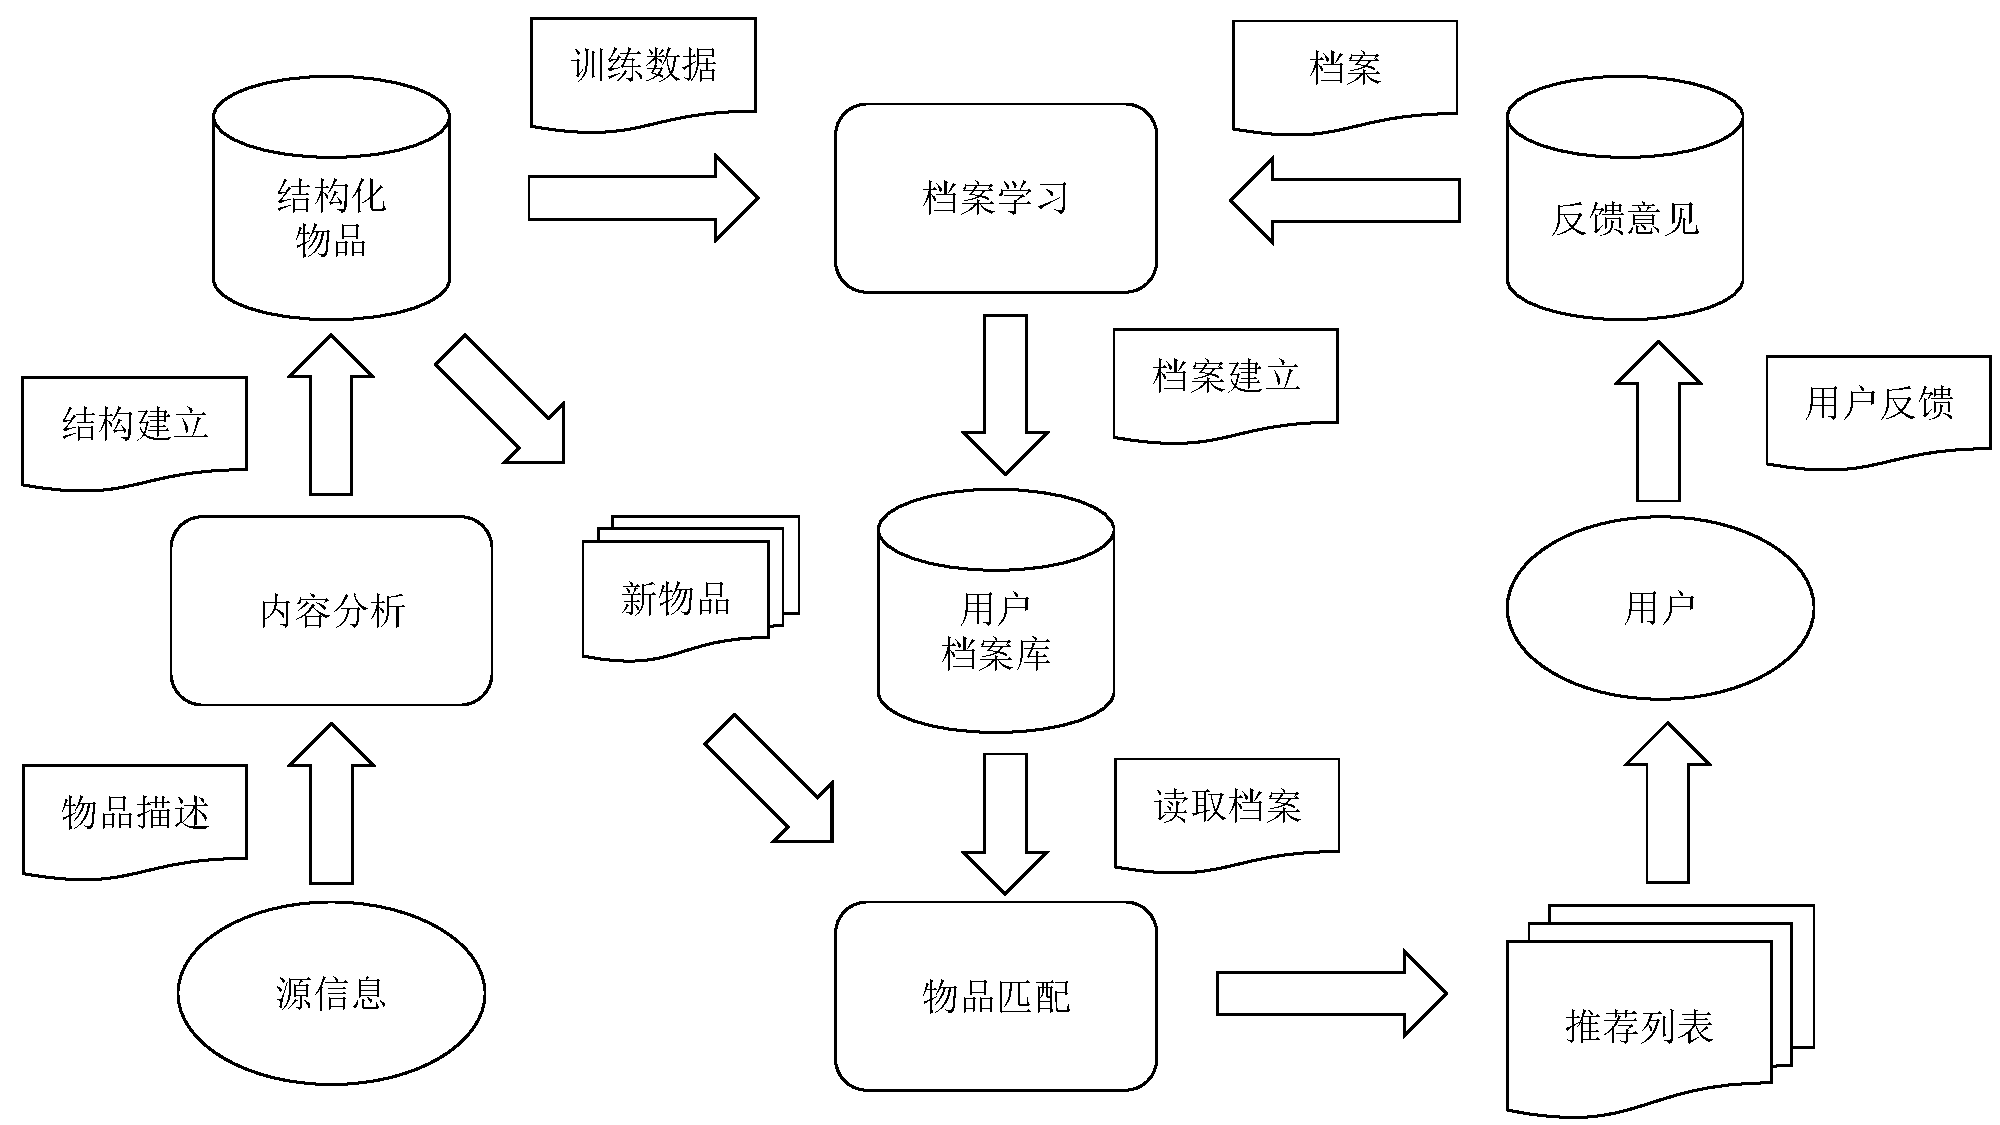
\includegraphics[width=0.75\linewidth]{02/1_cbr_arch.pdf}
 \bicaption[fig:cbr_arch]{推荐架构}{基于内容推荐算法的系统架构}{Fig}{Architecture of Content-based Recommender System}
\end{figure}

图\ref{fig:cbr_arch}展示了基于内容推荐算法的系统架构。其中椭圆形模块代表源数据,包括物品、用户信息;圆角矩形代表关键组件;圆柱形模块代表处理后的数据;箭头方向代表流程及数据流向。

在内容分析组件中,通常会借用信息检索系统中的技术,为源信息中的物品提取特征,生成物品描述以及物品的结构化内容,并将其进行存储。为了在偏好学习阶段对用户偏好模型进行创建及更新,需要存储用户对物品的评价。偏好学习组件基于用户的训练数据集,通常使用有监督学习算法建立用户偏好模型,并将该模型存储在模型仓库中。对于每一个结构化的物品,物品过滤组件会预测用户是否对该物品有偏好,将用户最可能偏好的$K$个物品生成一份推荐列表展示给用户。此外,用户的偏好可能会随时间改变,因此,系统还需维护用户的实时信息,如用户对推荐列表中物品的评价等。根据新生成的训练集,使用偏好学习组件对用户偏好进行自动更新。

\subsection{基于内容推荐系统的优点及缺点}

基于内容推荐系统的优点如下:

\begin{itemize}
 \item 用户独立性。基于内容推荐算法仅依据用户自己的评分记录建立其偏好模型。而基于协同过滤的方法需要其他用户的评分来为目标用户挑选出偏好最近邻的用户,也只能推荐近邻用户偏好的物品。
 \item 可解释性。通过列出物品特征,为用户对推荐物品做出解释。这些特征也可以作为衡量推荐系统准确性的标准,便于对内容分析策略进行调整。而在基于协同过滤的推荐算法中,唯一可以为用户进行解释就是另一个与目标用户偏好相似的用户也喜欢这个物品,缺乏可信度。
 \item 适用于物品冷启动。如果一项物品新加入到系统中,还没有被用户评分。基于协同过滤的推荐系统无法对此物品进行推荐。而基于内容的推荐系统可以克服物品冷启动问题。
\end{itemize}

同时,基于内容的推荐系统也有以下缺点:

\begin{itemize}
	\item 内容分析的局限性。基于内容推荐算法中的内容分析模块往往只能提取部分数量与类型的内容特征,这些特征是为用户建立偏好模型和进行物品推荐的主要依据。内容分析无法捕捉一些可能影响到用户购买决策的隐藏特征以及特征之间的关联。并且内容分析过程往往是领域相关的,通常需要丰富的专业领域知识。
	\item 过度匹配。基于内容推荐系统完全按照物品与用户偏好模型的匹配程度为物品进行打分、排序;并将排位较高的物品推荐给用户。因此,用户只能获取与其历史物品相似的推荐。推荐系统失去了新颖度。
	\item 用户冷启动问题。为了能够充分理解用户的偏好,建立有信服度的偏好模型。用户需要为一定数量的物品做出评价。因此,对于评价较少的新用户,系统难以给出可靠的推荐。
\end{itemize}

在机票推荐算法研究中,我们会在基于内容推荐的基础上,对物品内容分析及用户冷启动问题做出深入研究,以提升个性化机票推荐的效果。


\section{协同过滤推荐系统}

协同过滤推荐系统(Collaborative Filtering, CF)根据其他用户对物品的评价,为目标用户提供推荐。协同过滤的思想最早是在文档检索领域诞生的\cite{schafer2007collaborative},随着信息技术和互联网的发展,越来越多的诸如讨论帖、邮件清单等包含非正式内容的文档被收集到文档库中,用户难以快速了解文档的主题以及文档的质量水准,为文档检索带来了新的挑战。在二十世纪九十年代的研究发现,结合人工评价的半自动文档检索系统可以有效地解决该类问题。随后,结合人工干预的信息检索及推荐系统被大量研究\cite{goldberg1992using}。

协同过滤推荐系统的主要功能包括两个方面。第一是物品评价预测,其含义是对于一项用户未曾接触过的物品,预测用户对该物品的评价(喜好程度)。如果该物品新加入系统,缺乏用户行为记录,对其进行评价预测是较为困难的。第二是物品推荐,按照用户对物品的偏好程度,为其推荐一组物品。物品推荐通常建立在物品评价预测的基础上,除了以用户评价对物品进行排序之外,如何向用户展示推荐结果也是重要的考虑因素。近年来,协同过滤推荐领域有较多的研究成果,并且研究重心也从如何准确捕捉用户偏好转移到如何提升推荐算法的性能方面。本节我们主要介绍最常用的基于最近邻的协同过滤推荐算法。


\subsection{基于最近邻的推荐算法}
基于最近邻的推荐算法是协同过滤中最常用的方法之一,包括基于用户的最近邻算法和基于物品的最近邻算法两类。

基于用户的最近邻算法为目标用户根据相似的其他用户做出评价预测及物品推荐。首先需要建立用户间相似度的衡量方法。
\begin{equation}
\label{eq:user_sim}
	w(a,b) = \frac{\sum_j(v_{a,j}-\bar{v}_a)(v_{b,j}-\bar{v}_b)}{\sqrt{\sum_j(v_{a,j}-\bar{v}_a)^2\sum_j(v_{b,j}-\bar{v}_b)^2}}
\end{equation}

式\ref{eq:user_sim}衡量了用户之间的相似度。式中,$v_{a,j}$代表用户$a$对物品$j$的评分,$\bar{v}_a$代表用户$a$评价过的所有物品的平均评分。$j$代表用户$a$和用户$i$共同有过评分记录的物品。相似度$w(a,b)$的取值范围在$-1$到$1$之间。如果用户之间的相似度为负数,代表这两位用户之间的差异较大,在为用户挑选最近邻用户时通常会舍弃这部分用户。

\begin{equation}
\label{eq:rate_pred_ub}
	p_{a,i} = \bar{v}_a + \frac{\sum_{n \in neighbor(a)}w(a,n)(r_{ni} - \bar{r}_n)}{\sum_{n \in neighbor(a)}w(a,n)}
\end{equation}

式\ref{eq:rate_pred_ub}计算了评价预测的结果。第一项$\bar{v}_a$是目标用户的历史平均评分,第二项根据每位近邻用户的相似度以及这些用户的平均评分,对物品$i$进行评价。有些用户习惯为物品打高分,而有些用户习惯为物品打低分,公式使去中心化的方式适应用户的不同评价标准。

基于物品的最近邻算法根据用户记录中的相似物品,为用户进行评价预测及物品推荐\cite{sarwar2001item},可以认为基于物品的最近邻算法是基于用户的最近邻算法的转置。
\begin{equation}
\label{eq:item_sim}
	w(i,j) = \frac{\sum_u(v_{u,i}-\bar{v}_u)(v_{u,j}-\bar{v}_u)}{\sqrt{\sum_u(v_{u,i}-\bar{v}_u)^2\sum_u(v_{u,j}-\bar{v}_u)^2}}
\end{equation}

\begin{equation}
\label{eq:rate_pred_ib}
	p_{a,i} = \frac{\sum_{j \in relaitem(a)}w(i,j)r_{ai}}{\sum_{j \in relaitem(a)}w(i,j)}
\end{equation}

式\ref{eq:item_sim}和\ref{eq:rate_pred_ib}分别描述了物品间相似度和根据物品相似度为用户进行评价预测的方法。为了衡量物品$i$和$j$的相似度,需要使用对这两项物品都有过评价记录的所有用户评分,公式中同样进行了去中心化处理。

在最近邻推荐算法中,用户评价数据通常较稀疏。如果用户间共同评分记录的物品很少,或物品间有过共同评分记录的用户数量很少,他们容易得到很高的相似度,但这种相似度并不可靠。在系统实践中,通常仅考虑最近邻的$K$个用户或物品,并且增加一项评价记录数量的激励因子。
此外,对于流行度较高的物品,大多数用户对它的评价都很高,这类物品不具备很强的参考价值。一些协同过滤推荐算法\cite{breese1998empirical}对物品的流行度增加了惩罚项。

在系统性能方面,算法的时间复杂度与用户、物品、评价数量呈线性关系,因此需要对算法性能做进一步优化。通常系统不会维护全部用户对或物品对间的相似性,而在维持前$K$个相似项的基础上进行增量更新\cite{herlocker1999algorithmic}。此外,还可以对用户和物品进行聚类,快速定位与目标项相似的集合。

一些算法通过为物品降维的方式减少应用的复杂性,降维后的维度通常能够代表物品包含的主题特征,根据主题特征可以为用户的评价和他们潜在的偏好建立映射关系,进而根据用户的潜在偏好为其进行推荐。通过这种方法,物品评价预测往往可以在常数时间内完成。然而,这些方法在离线计算部分的时间复杂度很高,算法实现复杂,维护的成本也很高。常用的降维方法包括支持向量分解、主成分分析、特征提取等。

\subsection{协同过滤推荐的适用场景}

为了使协同过滤具备较好的推荐效果,本节对系统应具备的一些特性进行阐述,再结合本文的研究工作, 对协同过滤在机票推荐领域的应用进行分析。首先考虑数据的组织及形式,即数据分布特性:

\begin{enumerate}
  \item 系统包含一定数量的物品。如果系统中的物品较少,用户就可以自行了解每个物品,推荐系统的意义并不大。
  \item 每项物品具有一定数量的评价。如果物品收到的评价较少,则难以为用户提供可靠的预测与推荐。
  \item 用户评价条数远多于物品数量。根据协同过滤算法的原理,为了保障推荐效果,通常需要远多于物品数量的用户评价。通常,用户评价在物品中呈长尾分布,少量的热门物品拥有较多的评价,而大多数物品的评价数量较少。
  \item 物品持续性。在协同过滤系统中,用户需要分享他们曾经产生过评价的物品。在诸如新闻推荐等领域,物品的新鲜度往往只能持续数天。如果仅按照物品评价预测的结果对用户进行推荐,难以产生良好的推荐结果。
  \item 用户偏好持续性。协同过滤推荐在用户偏好不经常发生改变的领域具有较好的效果。否则,用户过去对物品的评价就不具备较高的参考价值。
\end{enumerate}

其次,协同过滤算法对系统还有一些潜在要求:

\begin{enumerate}
	\item 用户团体中存在偏好相似的用户。在团体中,与目标用户偏好相似的用户数量越多,协同过滤推荐的效果越好。反之,则难以产生预测与推荐。
	\item 物品的评价反映用户偏好。如果系统具备对物品评价的客观标准,协同过滤算法并不适用。然而,如果对物品的评价具有过强的主观性,或者具有多维度的评价标准,推荐系统需要对其进行整合与统一。
	\item 物品是同质的。系统中的物品应具备相同的本质特征,仅在用户的主观评价方面有所不同。协同过滤算法难以在不同质的物品间做出推荐。
\end{enumerate}

在机票推荐场景中,候选机票的数量很多,并且机票满足同质性。此外,用户的偏好具有较强的持久性。然而,在该领域直接应用协同过滤算法仍具有一定的挑战。首先,由于机票数量受限于航班的舱位,并且在起飞日期之前,机票的价格会产生较大幅度的持续波动,因此机票物品不具备较强的持久性。其次,用户对机票的评价较少且仅包含隐式正反馈评价,为协同过滤在机票推荐领域的应用带来了困难。

在本文的研究中,我们不直接向用户推荐机票,而是借鉴协同过滤的思路衡量航线及用户间的相似度,将协同过滤与基于内容的推荐结合起来,在冷启动场景下进一步提升机票推荐效果。

\section{主题模型}

随着网络上的信息以及专业文献库越来越丰富,自动从文本中抽取有效信息的技术变得更加重要。这类模型在文档标注、自动问答、自动生成摘要等应用场景起到很大作用。在信息检索、自然语言处理、机器学习等研究领域都对该类模型进行了深入研究。在起初几年,有监督的文档自动分类方法得到了很多的关注\cite{yang1999evaluation}。然而在很多情景下,文档库中的文档数量十分巨大,既没有预先定义的类别标签库,多数文档也没有标注类别标签。在诸如计算机、生物学等许多研究领域,文档的标签随着研究的进展发生很频繁的变化,对每篇文档进行人工标注也是不现实的。因而,基于无监督的文档模型具有更广阔的应用场景。

在研究实践中发现,基于生成模型\cite{zhong2005generative,hofmann1999probabilistic,blei2003latent,minka2002expectation}的统计方法对解决这类问题很有帮助。这类模型统称为主题模型。主题模型使用无监督策略从文档库中为每篇文档抽取可解释的表示模型。该模型将每篇文档表示成主题的混合分布,每个主题包括一组共同出现频率较高的词。主题可以将具有相似含义的词语联系到一起,还能为包含多种含义的词语确定在使用情境下的具体意义。在先前的研究中,最常见的文档表示方法是词袋模型(bag of words)\cite{zhang2010understanding}。这种模型将高维度的词汇向量转换到低维空间。综上,相比于其他的文档模型,主题模型有三点优势。第一,主题提取的过程是非监督的,即文档不需要标签以及初始化的步骤;第二,提取出的主题是可解释的,用户可以理解主题包含了哪些词汇;第三,每篇文档可以表示成多个主题的集合,可以捕捉主题之间的关系。


\subsection{主题模型概述}

主题模型的种类有很多。常见的方法包括潜在语义分析模型(LSA)、概率潜在语义分析模型(PLSA)以及潜在狄利克雷分布模型(LDA)等。

\subsubsection{LSA模型}
LSA\cite{deerwester1990indexing}的目的是为文档提取词汇的多重含义,并通过内容分析计算词汇以及文档之间的相似度。模型将文档库表示成一个矩阵,矩阵的每行代表一个词汇,每列代表一篇文档。矩阵的每个元素代表该词汇出现在文档中的频次。矩阵元素的值需要进行加权处理,考虑因素包括该词汇在文档中的重要程度以及该词汇在领域中总体信息丰富程度等。随后,对矩阵进行奇异值分解(singular value decomposition, SVD)\cite{higham2015singular}:
\begin{equation}
	A = U\sum V^T
\end{equation}

原矩阵$A$的维度是$M \times N$,分别是文档库中文档的数量以及词库的数量。矩阵$U$的维度是$M \times K$,矩阵$\sum$的维度是$K \times K$,矩阵$V^T$的维度是$K \times N$。其中$\sum$是一个对角矩阵,对角线的值由矩阵$A$的特征值组成。一般情况下,不需要使用矩阵所有的特征值,只需最大的前$K$个值就可以有效覆盖原矩阵的信息。矩阵$U$中的每列代表一个语义,每行代表一篇文档。每个元素代表该文档与该语义的相关程度;矩阵$V$中的每列代表一个关键词,每行代表一个词汇。每个元素代表该词汇与该关键词的相关程度;而中间的矩阵$\sum$的元素则表示语义和关键词之间的相关性。LSA将原本的文档特征进行降维,减轻了词汇和语义之间的复杂对应关系。

\subsubsection{PLSA模型}
PLSA是Hofmann\cite{hofmann1999probabilistic}在1999年提出了模型。该模型属于基于统计的潜在类别模型,使用了基于概率的生成模型对LSA进行改进。该模型的主要目标是区分词汇在不同语境上下文中的不同含义,主要包括两个方面,首先针对一词多义的情况下进行词义消歧;然后根据对在相同上下文中出现的单词进行聚类以揭示主题的概念。PLSA模型在诸如计算机视觉、推荐系统等领域中得到应用。

PLSA包含$K$个语义层面的隐式变量,我们称之为主题。则模型的变量包含三类。分别是文档集合$d \in D = \{d_1, \dots, d_n\}$;词汇集合$w \in W = \{w_1, \dots, w_m\}$;主题集合$z \in Z = \{z_1, \dots, z_k\}$。其中,文档和词汇是已知变量,主题是未知变量,$K$代表主题的数量,通常由先验决定。

\begin{figure}
 \centering
 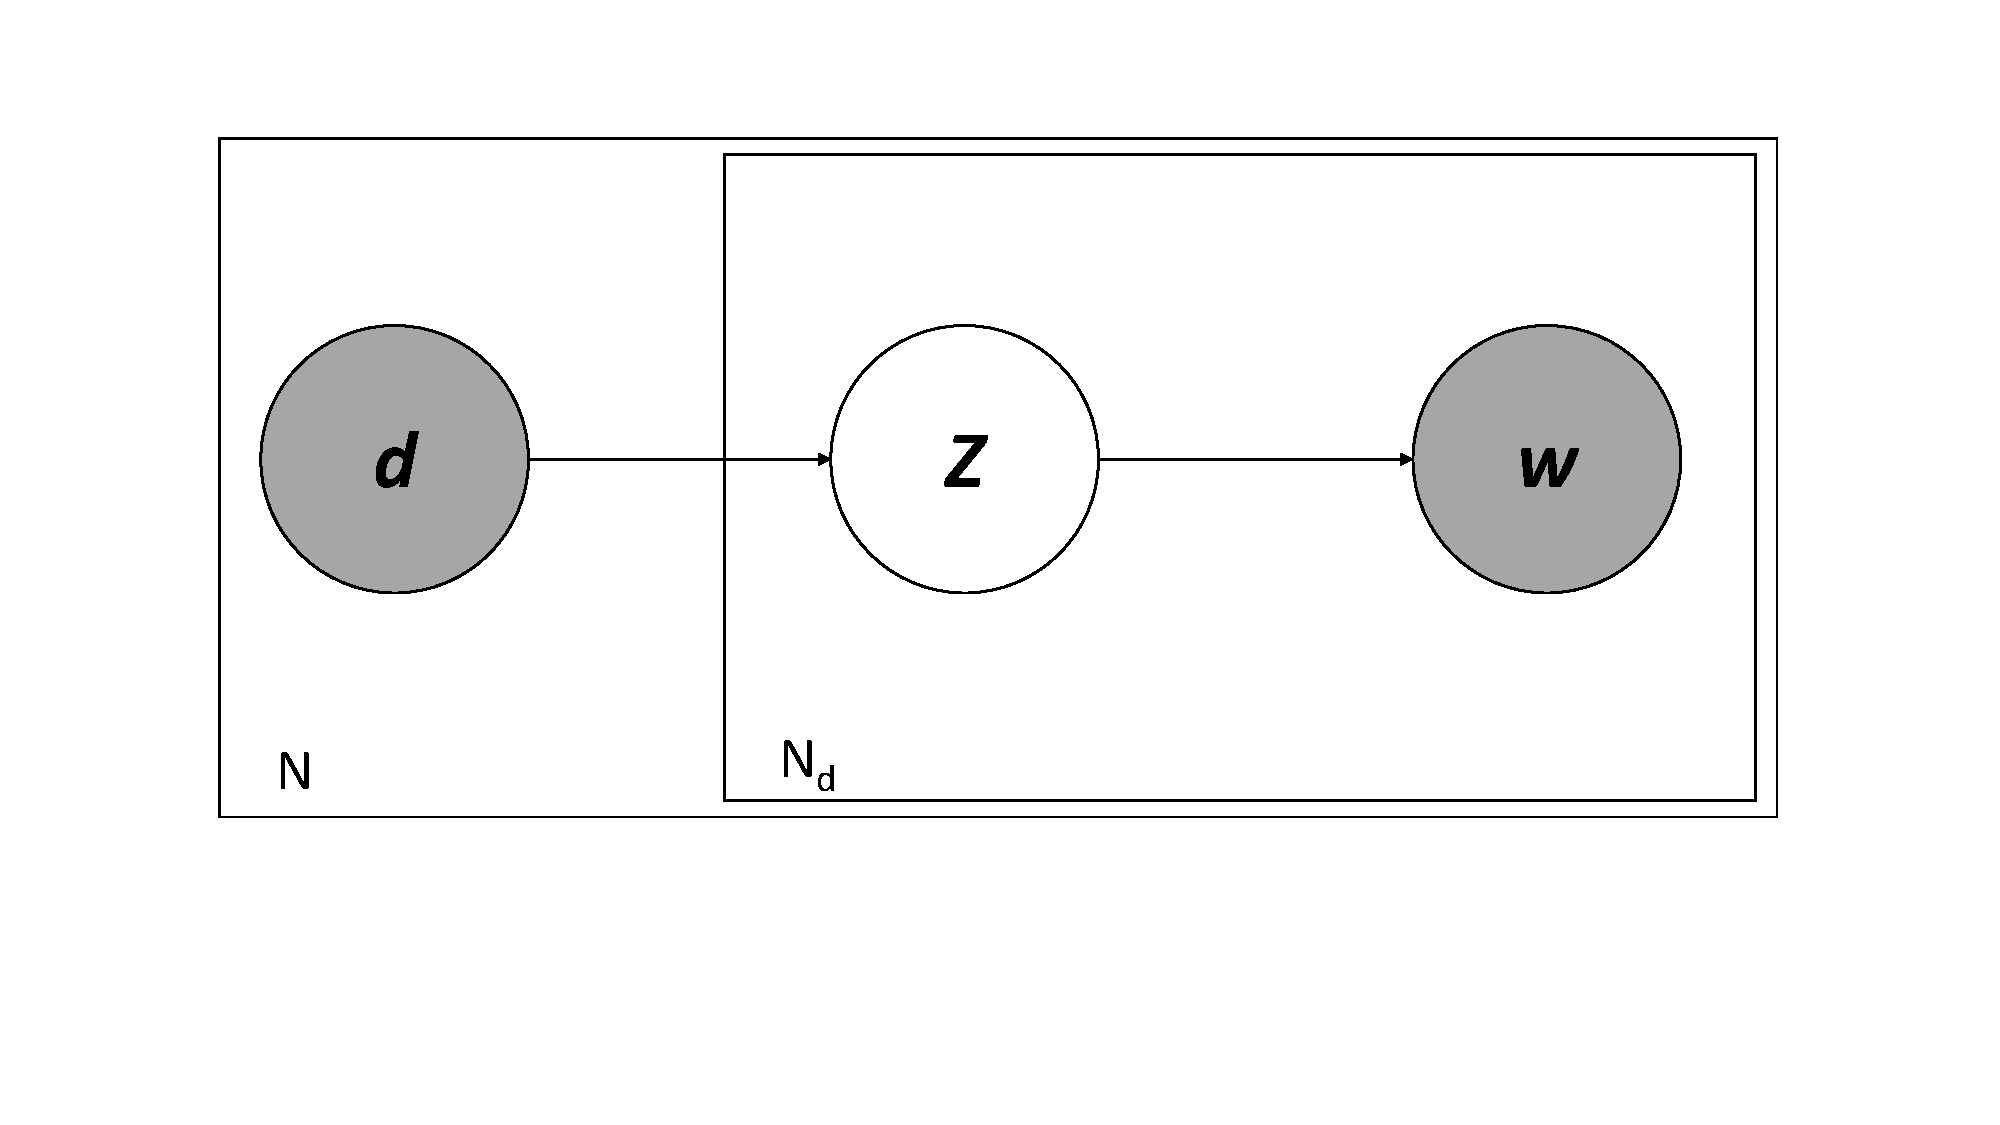
\includegraphics[width=0.7\linewidth]{02/2_plsa.pdf}
 \bicaption[fig:plsa]{PLSA}{PLSA概率图}{Fig}{Probability Graph for PLSA}
\end{figure}

图\ref{fig:plsa}是PLSA主题模型的概率图。$N$代指文档的数量,$N_w$代指每篇文档的词汇数量。带阴影的变量$d$,$w$分别代指文档与词汇,$z$代指隐式变量主题。每篇文档的生成过程描述如下:

\begin{enumerate}
\item 选择一篇文档 $d_n \sim P(d)$
\item 对于$d_n$中的每一个词汇
       \begin{enumerate}[fullwidth,itemindent=1em,label=(\alph*)]
       \item 基于多项式分布从文档中抽取主题,$z_i \sim P(z|d_n)$
       \item 基于多项式分布从主题中抽取词汇,$w_i \sim P(w|z_i)$
       \end{enumerate}
\end{enumerate}

一般情况下,我们可以认为对于给定的主题,词汇和文档是条件独立的,即$P(w|d,z) = P(w|z)$。则我们可以得到等式:
\begin{equation}
	P(w|d) = \sum_{z\in Z}P(w|z)P(z|d)
\end{equation}
\begin{equation}
	P(w,d) = \sum_{z\in Z}P(z)P(d|z)P(w|z)
\end{equation}

PLSA也可以应用在推荐系统中,将每位用户的历史购买记录视为一篇文档,购买过的没见物品视为一个词汇。可以根据模型分析出每篇文档与主题的关联。这里每个主题代表一种偏好习惯,根据每位用户的$P(z_k|d_i)$分布向量衡量用户相似度,就可以使用基于协同过滤的推荐算法。

\subsubsection{LDA模型}

在PLSA模型中,$P(z|d)$和$P(w|z)$都属于多项式分布,可以使用EM算法进行参数推导。但PLSA也有不足之处,首先参数$P(d)$是未知的,无法准确为一篇新文档设置概率值;其次,$P(z|d)$参数的数量随着文档的数量呈线性增长,可能会造成过拟合问题。

在LDA\cite{blei2003latent}模型中,同样有文档-主题分布矩阵$\Theta$和主题-词汇分布矩阵$\Phi$两个待估参数,这两个参数是分别服从超参数为$\alpha$和$\beta$的狄利克雷先验分布的随机变量。LDA与PLSA的不同之处在于:PLSA中,两个参数$P(z|d)$和P(w|z)是固定的未知变量。计算这两个变量的过程是先按照文档-主题和主题-词汇概率分布生成文档,再使用极大似然估计算法(如EM算法)对两个参数进行估计。但LDA模型将文档-主题和主题-词汇的概率分布视作服从狄利克雷先验分布的变量,而不是固定的值。通过这样设定参数,可以使用与狄利克雷分布共轭的多项式分布进行参数推导,并且还可以克服过拟合问题,比PLSA具有更好的效果。

\begin{figure}[!h]
 \centering
 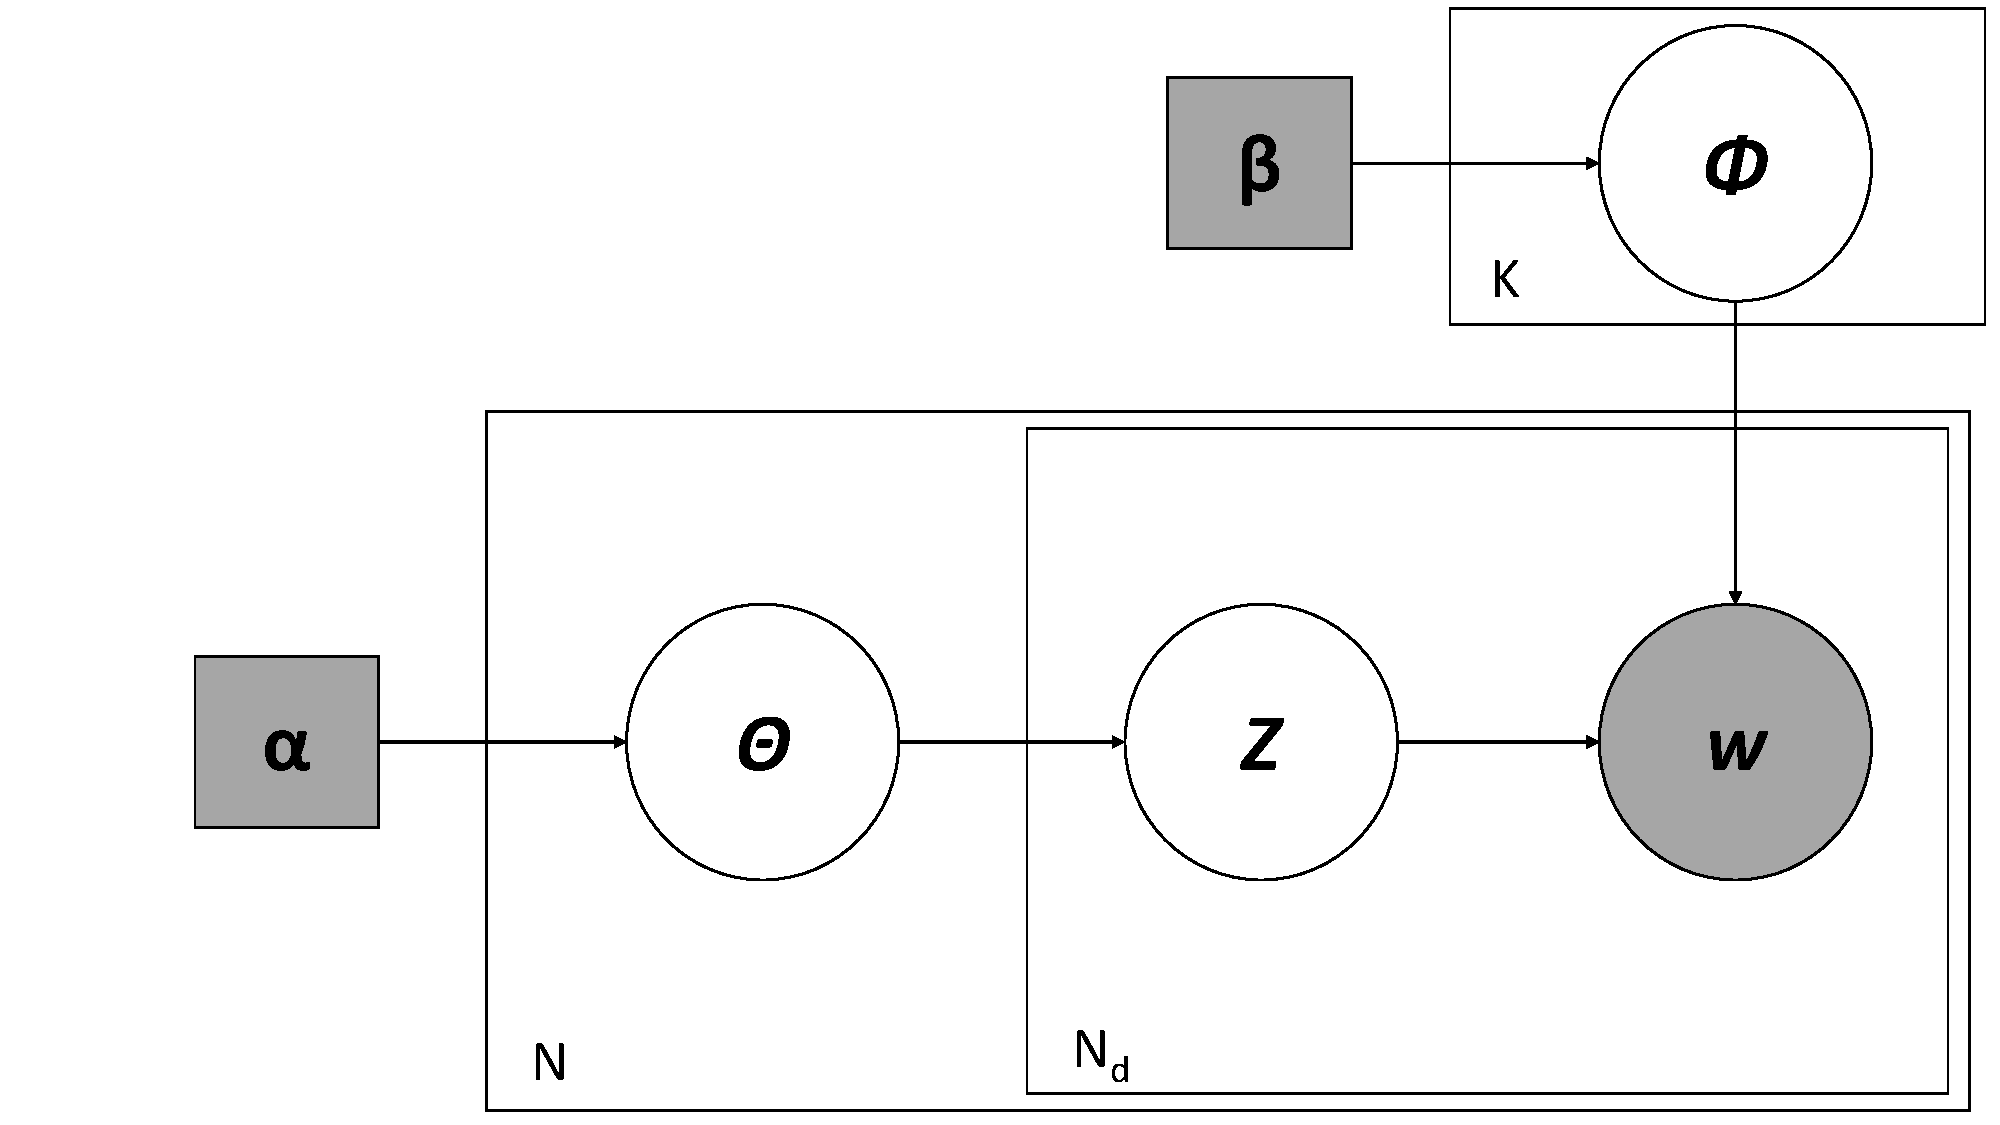
\includegraphics[width=0.7\linewidth]{02/3_lda.pdf}
 \bicaption[fig:lda]{LDA}{LDA概率图}{Fig}{Probability Graph for LDA}
\end{figure}

图\ref{fig:lda}是LDA主题模型的概率图。$N$代指文档的数量,$N_w$代指每篇文档的词汇数量,$K$代表主题的数量。带阴影的变量$\alpha$,$\beta$分别是两个待估参数的超参数,$w$代表词汇。每篇文档的生成过程描述如下:

\begin{enumerate}
\item 对每篇文档$d$,以狄利克雷先验初始化 $\theta_d \sim Dir(\alpha)$
\item 对每个主题$z$,以狄利克雷先验初始化 $\phi_z \sim Dir(\beta)$
\item 对于$d_n$中的每一个词汇
       \begin{enumerate}[fullwidth,itemindent=1em,label=(\alph*)]
       \item 基于多项式分布从文档中抽取主题,$z_i \sim Multi(\theta_{d_n})$
       \item 基于多项式分布从主题中抽取词汇,$w_i \sim Multi(\phi_{z_i})$
       \end{enumerate}
\end{enumerate}

LDA模型的参数具有超参数先验,如果先验足够准确,可以提升参数估计的准确率。并且适用于词汇数量较少的文档训练。此外,具有先验的参数可以对超参数进行调整,以适应不同的应用场景。在我们的研究中,使用主题模型来挖掘乘客和机票特征之间的关系,在共享账户情景中可以预测出乘客分布概率,以提升机票推荐的效果。


\iffalse
\section{模型参数估计}

在统计学中,参数估计\cite{heinrich2008parameter}代表使用样本数据来估计总体数据概率分布的过程。在机器学习模型中,参数往往用于描述模型的状态。而模型的真实分布是未知的,需要根据已知自变量和因变量之间的关系对整体模型的参数进行估计。一般使用独立同分布的数据集$\mathcal{X}$来表示随机变量$X$的一组观测值。$\theta$代指$X$的参数集合,取决于随机变量服从的分布。参数估计包括两个方面,第一类问题是估计参数$\theta$使得$\mathcal{X}$的出现概率最大;第二类问题是估计新的观测值$\tilde{x}$的概率。第一类问题是估计问题,而第二类问题是预测分类问题。

参数估计的方法有很多,本节我们主要介绍两种训练模型常用方法,分别是最大似然估计(Maximum Likelihood Estimation,MLE)\cite{johansen1990maximum}以及最大后验概率(Maximum a Posteri,MAP)\cite{gauvain1994maximum}。

\subsection{最大似然估计}

最大似然估计的目标是估计参数使其最大化似然函数。通常似然函数都有如下的形式:
\begin{equation}
\label{eq:ml}
	L(\theta|\mathcal{X}) = p(\mathcal{X}|\theta) = \bigcap_{x \in \mathcal{X}}{X=x|\theta} = \prod_{x \in \mathcal{X}}p(x|\theta)
\end{equation}

式\ref{eq:ml}是随机变量对于一组样本的似然函数,其中$L(\theta|\mathcal{X})$的含义是随机变量$X$产生样本$\mathcal{X}$的概率。在参数估计过程中,我们通常对似然函数取$\log$以简化计算过程,我们可以定义新的目标函数:

\begin{equation}
	\hat{\theta}_{ML} = \arg\max_\theta \mathcal{L}(\theta|\mathcal{X}) = \arg\max_\theta \sum_{x \in \mathcal{X}}\log p(x|\theta)
\end{equation}

在最大似然估计的过程中容易出现过拟合的问题。由于待估参数过于贴合观测样本的特征,将观测数据集中的噪声也作为模型特性进行学习,因而降低了模型的泛化能力。可以使用添加正则项的方式解决过拟合问题。于是目标函数可以更新为:

\begin{equation}
	\hat{\theta}_{ML} = \arg\max_\theta \sum_{x \in \mathcal{X}}\log p(x|\theta) + \lambda\sum_{j=1}^n\theta_i^2
\end{equation}

通常我们使用梯度下降算法进行参数训练。以梯度的负方向作为迭代方向,并确定学习速率。通过参数迭代使其逐步接近目标点。根据最优化理论,若优化目标函数是非凸的,则可能只得到局部极大似然。可以采取模拟退火思想以及进行多次初始化训练的方法克服这个问题。

对于新观测值问题,由观测样本集$\mathcal{X}$得到样本$\tilde{x}$的概率可以根据已估计的参数$\hat{\theta}_{ML}$获得:

\begin{eqnarray}
p(\tilde{x}|\mathcal{X})& = &\int_{\theta \in \Theta}p(\tilde{x}|\theta)p(\theta|\mathcal{X})d\theta \nonumber \\
& \approx &\int_{\theta \in \Theta}p(\tilde{x}|\hat{\theta}_{ML})p(\theta|\mathcal{X})d\theta = p(\tilde{x}|\hat{\theta}_{ML})
\end{eqnarray}


\subsection{最大后验概率}

最大后验概率与最大似然估计很相似。相比于最大似然估计,MAP为待估参数设置了先验分布$p(\theta)$。根据观测样本使待估参数达到最大后验概率,属于贝叶斯方法。新的目标函数如下:

\begin{eqnarray}
	\hat{\theta}_{MAP} &=& \arg\max_\theta p(\theta|\mathcal{X}) \nonumber \\
	&=& \arg\max_\theta \frac{p(\mathcal{X}|\theta)p(\theta)}{p(\mathcal{X})} \nonumber \\
	&=& \arg\max_\theta {\sum_{x \in \mathcal{X}}\log p(x|\theta) + \log p(\theta)}
\end{eqnarray}

可以看出,相比于MLE的目标函数,最大后验概率的目标函数增加了一项先验分布。这项先验分布可以用来挖掘观测集额外的信息,也可以用于预防过拟合问题。在贝叶斯方法中,参数$\theta$也认为是随机变量,而不是固定的未知数值。通常使用超参数为$\theta$设置先验。参数的训练方法与MLE类似,都可以使用梯度下降法。对于新观测值的概率,同样使用已估计的参数$\hat{\theta}_{MAP}$得到。

\begin{equation}
p(\tilde{x}|\mathcal{X}) \approx \int_{\theta \in \Theta}p(\tilde{x}|\hat{\theta}_{MAP})p(\theta|\mathcal{X})d\theta = p(\tilde{x}|\hat{\theta}_{MAP})
\end{equation}
\fi

\section{本章小结}
本章介绍了与论文研究工作相关的一些技术。首先介绍了基于内容推荐系统,分析了该系统的系统架构及流程,还分析了基于内容推荐算法的优势与劣势。其次介绍了协同过滤推荐技术,介绍了基于最近邻的协同过滤推荐算法以及算法的适用场景。同时结合本文工作,分析了在机票推荐领域应用基于内容推荐和协同过滤推荐的挑战性。最后介绍了主题模型,分析了三类常用的生成模型,包括它们的参数推导、生成过程等。这三种技术为我们后续章节的研究做了理论铺垫。









